\documentclass[
	%a4paper, % Use A4 paper size
	letterpaper, % Use US letter paper size
]{jdf}


\author{Shashvat Sinha}
\email{shashvat.sinha@gatech.edu}
\title{Assignment M4 (Summer 2020)\\CS6750}

\begin{document}
%\lsstyle

\maketitle

\begin{abstract}
    For my \textbf{M*} assignments in CS6750 (Summer 2020), I have chosen to redesign the interface that \textbf{LinkedIn} uses for its messaging. There are several aspects of the messaging interface that, in my opinion, could be improved - there is limited support for threading, messages do not support rich text, and the editor is geared towards short texts rather than a proper messaging platform. 
    
    As a networking tool LinkedIn would benefit from improved communication between its users, as it would improve the value proposition its users see. By the end of the M* assignments, I plan to focus on the task of communicating using LinkedIn messaging, taking it  through a complete design lifecycle. 
\end{abstract}

\section{Qualitative Evaluation}
For the Qualitative Evaluation we shall select the \textbf{Think-Aloud Protocol}. This will be applied on the Verbal Prototype of the LinkedIn Messaging Search and Filtering capability that we are desiging as part of the M* assignments.

\subsection{Evaluation Plan}
\subsubsection{Participants}
We shall select 4 participants from friends and colleagues. 

\subsubsection{Recruitment}Participants will be recruited by gauging their interest in taking part in this study and their engagement with LinkedIn as a service.

\subsubsection{Location}
The evaluation will take place on Zoom. If the participants do not object, the calls will be recorded on Zoom, else the participant responses will be noted down.

\subsection{Evaluation Content}
\subsubsection{Directions to Participants}
\begin{enumerate}
    \item Participants will be given a brief on the M* projects, along with a recital of the abstract. 
    \item Depending on the interest level of the participants, the previous M* assignments will be shared with them, so as to bring them up to speed with the needs of this evaluation. 
    \item A walk-through of the Verbal Prototype will be given to the participants as described in M3.
    \item Finally, participants will be asked to imagine themselves in the position of using the prototype as described and verbalize their actions and thoughts on those actions.
\end{enumerate}


\subsubsection{Questions}
There will be no planned questions for the participants. There will however be questions to elicit detailed responses of their Think-Alouds where necessary.

\subsection{Evaluation Assessment}
Our \textbf{Requirements Definition} in M2 described the context aware search functionality as the following user story:

\hangindent=1.5cm
\hangafter=0
\textbf{As a} user looking for a specific contact or message thread
\textbf{I want to} be able to search for messages based on context (e.g. tags, subjects, projects, dates), content and sender or recipient filtering 
\textbf{such that} it is easy to find prior messages an threads based on what I remember about them (e.g. find me mails send in 2018 on a a job in San Francisco sent to persons with the last name 'Cook' or 'Jobs').

Therefore, to establish whether the verbal prototype has met the requirements above, the participants Think-Aloud process should have covered the specific expectations that are in the user
story above.
\begin{enumerate}
    \item Can I search for a message based on context
    \item What kinds of items do users think of under "context" and does the prototype allow for such a search.
    \item Can I find prior messages in older threads based on specific criteria
    \item What kinds of criteria do the participants expect, and does the verbal prototype make allowances for that?
\end{enumerate}

\section{Empirical Evaluation}
We shall Emperically Evaluate the Wireframe Prototype of the Messaging Window Layout.


\begin{figure}[h]
	\centering
	\frame{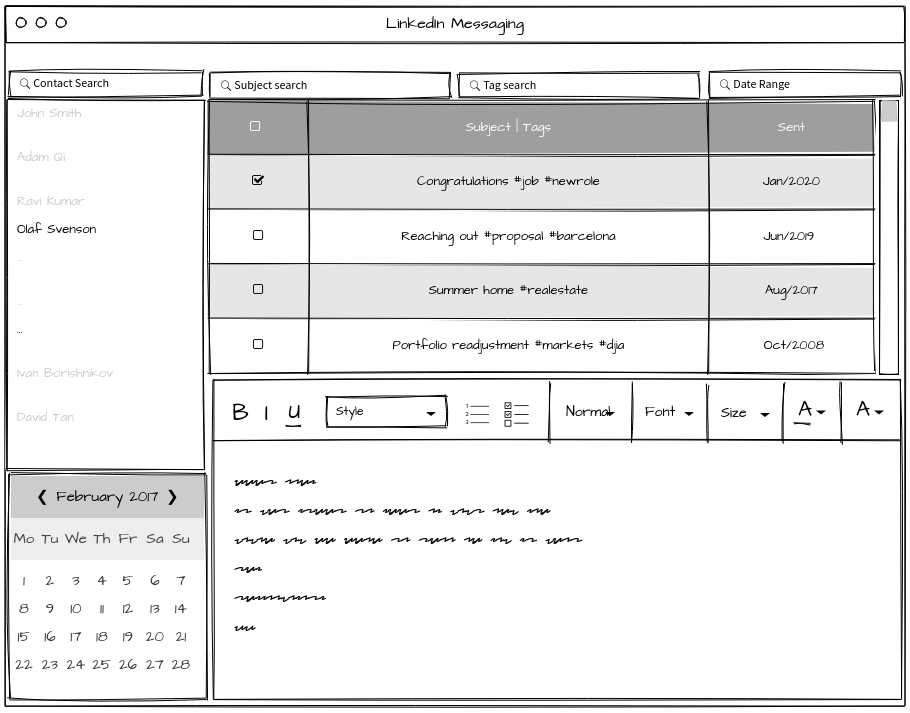
\includegraphics[width=14cm]{jdf-master/Figures/Message_Layout.png}}
	\caption{Messaging Window Layout}
	\label{fig:layout}
\end{figure}




\subsection{Controls}
We will be testing the ability of the user to do the following tasks with the prototype of the redesign of the LinkedIn Messaging Interface:
\subsubsection{Evaluation Items}
\begin{itemize}
    \item It should be easier for a user to navigate to the Messaging feature in LinkedIn
    \item It should be clearer how to select a user to send a message to.
    \item It should be clearer to find a specific thread to send a message to
    \item It should be faster to start writing a message given a specific user and a specific thread.
\end{itemize}

\subsubsection{Point of Comparison}
The point of comparison will be with the existing LinkedIn Interface.

\subsubsection{Null Hypothesis}
The null hypothesis is that the redesigned interface provides no improvement in efficiency over the current LinkedIn messaging interface as of July 2020.

\subsubsection{Alternative Hypothesis}
The alternative hypothesis is that the redesigned interface makes it faster for the user to action the items for evaluation as listed above.

\subsubsection{Experimental Method}
\begin{itemize}
    \item Our experimental method will be within-subjects. 
    \item Participants will work on the tasks individually.
    \item The participants in our evaluation will be given the list of tasks above and shown the existing LinkedIn interface. They will be asked to describe step by step how they will achieve those tasks. 
    \item Their descriptions will be timed. 
    \item Timings data will be compared between both interfaces.
\end{itemize}

\subsubsection{Confounding Variables}
One can expect that descriptive walkthroughs of static interfaces will not provide the same timing data as the actual usage of usable interfaces. 

\textit{Therefore, in order to do a like for like comparison, since the participants will be using a static wireframe prototype of the redesigned interface, they will also be shown a static screenshot of the existing interface}.

Thus we hope that both existing and prototype interfaces will be subject to the same variance. Since we are only interested in the delta between them, the variance from actual performance should cancel out.

\section{Predictive Evaluation}
For the predictive evaluation, we will perform either a cognitive walkthrough of our prototype

The users goals will be to select a thread and user to send a message to using the redesigned LinkedIn Messaging interface.

We will be evaluating a user’s navigation around the interface to figure out how to accomplish their goal. It is assumed that the user is coming to the messaging interface with a specific intent - to send a message on a specific thread to a specific person. The question is, how easy is it for them to do.


\section{Preparing to Execute}
We shall execute the following two evaluations in the next assignment:
\begin{itemize}
    \item The qualitative evaluation using the Think-Aloud protocol
    
    \textbf{Because} this evaluation allows for rich interaction with the users, which has been missing during M* assignments, and I would like to take the opportunity to discuss my redesign with peer users of LinkedIn.
    \item The predictive evaluation using a walkthrough
    
    \textbf{Because} this is something that I have attempted superficially, but was intrigued by the rigor expected as per Dr. Joyner's lecture on this topic.
\end{itemize}





\section{References}

\printbibliography[heading=none]


\end{document}